%& -shell-escape
%%% Copyright (c) 2011, Илья w-495 Никитин
%%%
%%% Разрешается повторное распространение и использование как в виде исходного
%%% кода, так и в двоичной форме, если таковая будет получена, 
%%% с изменениями или без, при соблюдении следующих условий:
%%%
%%%     * При повторном распространении исходного кода должно оставаться
%%%       указанное выше уведомление об авторском праве, этот список условий и
%%%       последующий отказ от гарантий.
%%%     * Ни имя w-495, ни имена друзей или консультантов не могут быть
%%%       использованы в качестве поддержки или продвижения продуктов,
%%%       основанных на этом коде без предварительного письменного разрешения. 
%%%
%%% Этот код предоставлен владельцом авторских прав и/или другими
%%% сторонами "как она есть" без какого-либо вида гарантий, выраженных явно
%%% или подразумеваемых, включая, но не ограничиваясь ими, подразумеваемые
%%% гарантии коммерческой ценности и пригодности для конкретной цели. Ни в
%%% коем случае, если не требуется соответствующим законом, или не установлено
%%% в устной форме, ни один владелец авторских прав и ни одно  другое лицо,
%%% которое может изменять и/или повторно распространять программу, как было
%%% сказано выше, не несёт ответственности, включая любые общие, случайные,
%%% специальные или последовавшие убытки, вследствие использования или
%%% невозможности использования программы (включая, но не ограничиваясь
%%% потерей данных, или данными, ставшими неправильными, или потерями
%%% принесенными из-за вас или третьих лиц, или отказом программы работать
%%% совместно с другими программами), даже если такой владелец или другое
%%% лицо были извещены о возможности таких убытков.


% Оный документ нужно собирать только в XeTeX
% Командой:
% 	>xelatex имя-файла.tex
% Для этого должен быть установлены пакеты XeLaTex и XeTeX
% в TeXLive или MikTeX или иной, если она поддерживает последние обновдения CTAN


\documentclass[unicode, 14pt, a4paper,oneside,fleqn]{extarticle}
	%% Варианты []:
		% fleqn --- сдвигает формулы влево

	%% Варианты {}:
		% book
		% report
		% article
		% letter
		% minimal (???)
		
\usepackage{setspace}
\onehalfspacing

\usepackage{styles/init} 
	% Подключаем набор стилей.
	% Там были определены базовые настройки шрифтов
	% 	и пакетов роботы с графикой и листингами.
	
	% При не обходимости шрифты следует переопределить.
	% Если в Вашей системе не окажется нужных шрифтов, pdf не соберется.


\begin{document}


%%%%%%%%%%%%%%%%%%%%%%%%%%%%%%%%%%%%%%%%%%%%%%%%%%%%%%%%%%%%%%%%%%%%%%%%%%%%%%%%
%%%
%%% бесполезное содержимое
%%%

	\begin{titlepage}
\begin{center} %% ПО ЦЕНТРУ

\bfseries
%%%%%%%%%%%%%%%%%%%%%%%%%%%%%%%%%%%%%%%%%%%%%%%%%%%%%%%%%%%%%%%%%%%%%%%%%%%%%%%%
%%%
%%% ВУЗ
%%%

	{\Large Национальный исследовательский университет  \\
	Высшая Школа Экономики
	
	} %% или что-то в этом духе

\vspace{48pt}

%%%%%%%%%%%%%%%%%%%%%%%%%%%%%%%%%%%%%%%%%%%%%%%%%%%%%%%%%%%%%%%%%%%%%%%%%%%%%%%%
%%%
%%% Факультет
%%%

	{\large Факультет Компьютерных Наук
	
	}

	%{\large Факультет иностранных языков
	%
	%}

\vspace{12pt}
%%%%%%%%%%%%%%%%%%%%%%%%%%%%%%%%%%%%%%%%%%%%%%%%%%%%%%%%%%%%%%%%%%%%%%%%%%%%%%%%
%%%
%%% Кафедра
%%%


	{\large  { Прикладная Математика и Информатика}
	
	} %% или что-то в этом духе

\vspace{72pt}
%%%%%%%%%%%%%%%%%%%%%%%%%%%%%%%%%%%%%%%%%%%%%%%%%%%%%%%%%%%%%%%%%%%%%%%%%%%%%%%%
%%%
%%% Класс работы
%%%

	{\Huge Выявление токсичного контента на портале для обмена знаниями Quora
	
	}
	% Лекции по курсу \enquote{Какой-то предмет} 
	% Лабораторная работа по курсу \enquote{Какой-то предмет} 
	% Курсовая работа по курсу \enquote{Какой-то предмет} 
	% Курсовой проект по курсу \enquote{Какой-то предмет} 

\vspace{12pt}
%%%%%%%%%%%%%%%%%%%%%%%%%%%%%%%%%%%%%%%%%%%%%%%%%%%%%%%%%%%%%%%%%%%%%%%%%%%%%%%%
%%%
%%% Название работы
%%%

	%{\Large <<Какое-то название>> 
	%}

\end{center} %% УЖЕ НЕ ПО ЦЕНТРУ

\vspace{60pt}
%%%%%%%%%%%%%%%%%%%%%%%%%%%%%%%%%%%%%%%%%%%%%%%%%%%%%%%%%%%%%%%%%%%%%%%%%%%%%%%%
%%%
%%% Автор(ы)
%%%

	\begin{flushright}
		\begin{tabular}{rl}
			Преподаватель: & Д.\,И. Игнатов \\
			Студент: & Е.\,А. Казаков \\
		\end{tabular}
	\end{flushright}

\vfill
%%%%%%%%%%%%%%%%%%%%%%%%%%%%%%%%%%%%%%%%%%%%%%%%%%%%%%%%%%%%%%%%%%%%%%%%%%%%%%%%
%%%
%%% Дата
%%%

	\begin{center} %% ПО ЦЕНТРУ
		\bfseries
		Москва, 2019
	\end{center}
	
\end{titlepage} 

 	% титульный лист
	\tableofcontents 		% оглавление
	\pagebreak

	%%%%%%%%%%%%%%%%%%%%%%%%%%%%%%%%%%%%%%%%%%%%%%%%%%%%%%%%%%%%%%%%%%%%%%%%%%%%%%%%
	%%%
	%%% дополнительное (свое) задание верхнего колонтитула
	%%% 
	%%%
	%	\makeatletter
	%	\renewcommand{\@oddhead}{ \textcolor{blue}{Лекция (задача) \arabic{lections}} \hfil \par
	%	\hfil  \leftmark \hfil \rightmark }
	%	\makeatother

	
%%%%%%%%%%%%%%%%%%%%%%%%%%%%%%%%%%%%%%%%%%%%%%%%%%%%%%%%%%%%%%%%%%%%%%%%%%%%%%%%
%%%
%%% полезное содержимое
%%%
	
		\section{Введение}

\subsection{Аннотация}
    В качестве объекта исследования в рамках курсовой работы мной был выбран кейс, предложенный известным порталом по обмену знаниями Quora. На протяжении всего своего существования Quora сталкивается с нежелательным контентом, который ухудшает пользовательский опыт и усложняет работу всего сайта. Моя задача состоит в том, чтобы разработать универсальную расширяемую многофункциональную систему для распознавания и отсеивания такого токсичного контента.\\
    
    As an object of study in the course work I have chosen the case proposed by the well-known portal for the exchange of knowledge Quora. Throughout its existence, Quora encounters unwanted content that degrades the user experience and complicates the operation of the entire site. My task is to develop a universal expandable multifunctional system for the recognition and screening of such toxic content.
\subsection{Актуальность}

    Трудно переоценить своевременность и актуальность поднимаемой проблемы: каждый из нас каждый день сталкивается с неподобающим поведением со стороны других пользователей интернета. В основном, это вызвано анонимностью оставленных комментариев, однако мы не пойдем по пути деанонимизации, а будем бороться с проблемой путем автоматического определения и удаления спорного содержания. Полученное решение без проблем можно обобщить на другие области, например комментарии в соцсетях, отзывы на товары и т.п.

\subsection{Структура работы}

    	Моя работа будет разбита на две смысловые части. В первой мы подберем математическую модель, которая бы лучше всего подходила для поставленной задачи и достигала требуемого качества. Мы рассмотрим несколько вариантов решения и выберем лучший из них.
    	
    	Во второй части мы сконцентрируемся на реализации выбранной модели. Рассмотрим общие архитектурные решения для задач по машинному обучению и обработке данных, обозначим проблемные моменты, которые помешают масштабированию проекта, и в конечном итоге придем к наиболее удобной структуре проекта, которая бы поддерживала работу с несколькими математическими моделями, преобразователями данных, инструментами для статистического анализа и т.п.
\pagebreak
\subsection{Обозначения}
На протяжении всей работы я буду сопровождать текстовые выкладки иллюстрациями в виде блок-схем. В целом, обозначения в них довольно очевидны, однако, чтобы исключить неправильное понимание, уточним их.
Они будут состоять из следющих объектов:

\begin{table}[ht]
\caption{Обозначения в блок-схемах}
\centering
\begin{tabular}{*{2}{m{0.48\textwidth}}}
\hline
\begin{center}
\includegraphics[height=40pt]{images/raw_digram_example}\end{center}&Необработанные данные, поступающие на вход программы. В случае с решением задачи от Quora ими являются формулировки вопросов, которые нужно профильтровать.\\\\
\begin{center}
\includegraphics[height=36pt]{images/transformed_data_example}\end{center}&Данные, полученные нами из исходных некоторым преобразованием. Например, это может быть лемматизированный текст или вектор, характеризующий относительное семантическое положение слова.\\\\
\begin{center}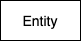
\includegraphics[height=30pt]{images/entity_example}\end{center}&Абстрактная сущность, которая в нашей архитектуре будет выполнять поставленную ей роль.\\
\end{tabular}
\label{tab:gt}
\end{table}

Как можно видеть, схемы довольно простые, и, в тоже время, функциональные.
\pagebreak
	%% Cильный и слабый пределы
		\section{Постановка задачи}


\subsection{Условие}
Остановимся подробнее на задаче, поставленной перед нами. Формально, это проблема о классификации текстовых вопросов на два класса: \textbf{разрешенный контент}, \textbf{токсичный контент}. Существует довольно полное определение токсичности, которое Quora приводит в условии:

\begin{itemize}
\item
Не нейтральный тон
\subitem
    -- Намеренное преувеличение направленное на подчеркивание определенной точки зрения
\subitem
    -- Риторический вопрос, не предполагающий конкретного ответа
\item Пренебрежение и/или оскорбление
\subitem
    -- Дискриминационные высказывания, поощрение стереотипов о незащищенных группах
\subitem
    -- Пренебрежение и/или оскорбление в адрес конкретного человека или группы людей
\subitem
    -- Клевета или основанная на неподтвержденных фактах информация в отношении конкретного человека или группы людей
\item Очевидно ложные высказывания
\item Запрещенные темы
\subitem
    -- Темы 18+
\subitem
    -- Политика
\subitem
    -- Жестокое обращение с животными

\end{itemize}

\pagebreak

\subsection{Входные данные}

Организаторы данного kaggle-соревнования предлагают следующий набор датасетов:
\begin{itemize}
\item \textbf{train.csv} - данные для обучения, для которых известен результат идеальной классифицирующей модели. Представляет из себя csv-файл, в первой колонке которого содержится uuid вопроса, во второй - текстовая формулировка, в третьей - класс, к которому пренадлежит вопрос.

\item \textbf{test.csv} - данные, для которых необходимо предсказать классификацию. Представляет из себя csv-файл, в первой колонке которого содержится uuid вопроса, во второй - текстовая формулировка.\\

\item \textbf{GoogleNews-vectors-negative300.bin} - словарь векторизации слов, построенный на корпусе текстов GoogleNews. Размерность векторов - 300.
\item \textbf{glove.840B.300d.txt} - словарь векторизации слов, построенный на корпусе текстов Glove [4]. Размерность векторов - 300.
\item \textbf{paragram\_300\_sll999.txt} - словарь векторизации слов, построенный на корпусе текстов Paragram. Размерность векторов - 300.
\item \textbf{wiki-news-300d-1M.vec} - словарь векторизации слов, построенный на корпусе текстов Wiki News. Размерность векторов - 300.
\end{itemize}

По предоставленному набору данных можно понять, что организаторы предлагают в решении подумать в сторону векторизации слов, используя эти словари. Хорошая идея, вернемся к ней позже.


\pagebreak





	%% Спектр оператора
		\section{Существующие решения}

Проблема выявления токсичного контента актуальна с самого основания сети Интернет. И, конечно, уже существует большое количество решений, помогающих в этом. Давайте рассмотрим наиболее распространенные из них.
 
\subsection{Perspective API}
  
Один из самых известных проектов на эту тему - разработка 2017 года, принадлежащая компании \textbf{Google} под названием \textbf{Perspective API}.

Авторы ставили перед собой задачу создать инструмент для модераторов, позволяющий обрабатывать комментарии на крупных платформах, таких как \textbf{Reddit}, \textbf{9gag}, и т.п. Среди партнеров также значатся крупные новостные агенства \textbf{The New York Times}, \textbf{The Guardian}, \textbf{The Economist}, и т.п.

К сожалению, мне не удалось найти подробное описание алгоритма, который используют разработчики этого сервиса. Вся общедоступная информация о технической части состоит только в том, какие корпусы текстов использовались для обучения модели.

\subsection{Scale Text Classification}

Сервис от компании \textbf{Scale} не направлен конкретно на работу с токсичным контентом. Однако, он считается одним из самых удачных в плане классификации на тематические классы. Таким образом, используя его, можно захватить все запрещенные к публикации группы контента.

Как и в предыдущем случае, код и алгоритмические наработки являются собственностью компании и закрыты для широкого пользования. Поэтому мы не будем долго останавливаться на нем.

\subsection{Соревнования на Kaggle}

Контест, организованный компанией \textbf{Quora} далеко не первый, связанный с классификацией токсичного контента. Как пример можно привести соревнование 2018 года от компании \textbf{Jigsaw}. Очень часто участники высоких мест выкладывают разборы своих решений, в которых рассказывают основное устройство модели и проблемы, с которыми они столкнулись в процессе исследования. Для нашей задачи полезно будет ознакомиться и разобраться в том, какие методики использовали участники, добившиеся наибольших результатов.

Я проанализировал несколько таких разборов, и пришел к выводу о том, что главный прирост в качестве дает использование словарей векторизации совместно с рекуррентными сетями. Таким образом мы можем заключить, что стоит подумать в направлении использования рекуррентных сетей применительно к текстам вопросов.

В целом, это довольно очевидный вывод, и хорошо, что разбор аналогичных задач подтвердил его.



\pagebreak





	%% Спектр оператора
		

%%%%%%%%%%%%%%%%%%%%%%%%%%%%%%%%%%%%%%%%%%%%%%%%%%%%%%%%%%%%%%%%%%%%%%%%%%%%%%%%
%%%
%%% тема лекции
%%%

\section{Теория}

\subsection{Обработка данных}

В качестве препроцессинга данных и приведения их к удобоиспользуемому виду я предлагаю использовать стандартный подход \textbf{word embedding}. Он заключается в том, что каждому слову сопоставляется вектор в некотором многомерном векторном пространстве. Чаще всего вектор подбирают таким образом, чтобы они каким-то образом характеризовали семантическое положение слова относительно остальных.

\begin{center} 
\includegraphics[width=370pt]{images/model_schema_1.png}\end{center}

Довольно известен пример такого проецирования из работы Томаша Миколова [2, 3], одного из основоположников теории world2vec.

\begin{center} 
\includegraphics[width=300pt]{images/model_schema_2.png}

Можно видеть, что взаимное расположение\\ \textbf{Woman} и \textbf{Man} близко к \textbf{Queen} и \textbf{King}, \textbf{Aunt} и \textbf{Uncle}.\end{center}

В рамках этой работы мы не будем рассматривать способы проецирования слов в векторное пространство. Мы возьмем уже готовые широкоиспользуемые словари, подготовленные на основе больших корпусов текстов: \textbf{glove}, \textbf{wiki-news}, \textbf{GoogleNews}, \textbf{paragram}.

Наш \textbf{word embedding} для конкретного слова будет представлять собой конкатенацию векторов из всех этих словарей. Предполагается, что полученные таким образом векторы будут давать хорошую возможность для обучения описанной далее модели.

\subsection{Модель}

Обозначим требования к модели, которая должна получиться в результате:
\begin{itemize}
    \item Способность выделять тему, контекст и ключевые слова в предложении
    \item Обладание долговременной памятью о предыдущих предложениях
    \item Обладание кратковременной памятью о предыдущих словах при их последовательной обработки
\end{itemize}


\subsubsection{Нейронная сеть}
Рассмотрим обычную нейронную сеть. Как мы знаем, общих чертах она представляет из себя набор слоев из нейронов,  последовательно соединенных друг с другом. На вход она принимает вектор, пропускает его значения через все связи с весами, вычисленными в процессе обучения и в выходном слое выдает некоторую величину.

\begin{center} 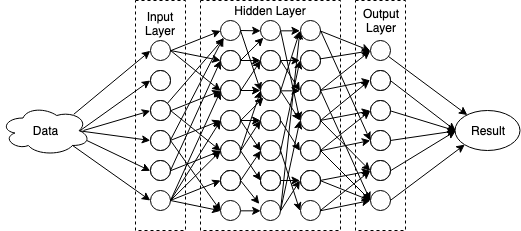
\includegraphics[width=450pt]{images/model_schema_3.png} \end{center}

Однако без доработок эта модель не запоминает свои предыдущие решения, а работает только в текущем контексте. Для исправления этого недостатка была разработана теория рекуррентных сетей.


\subsubsection{Рекуррентная сеть}

В рекуррентной сети добавляется сохранение некоторых состояний и передача их в дополнительным входным потоком при последующих запусках: 

\begin{center} 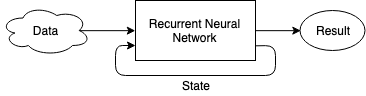
\includegraphics[width=330pt]{images/model_schema_4.png} \end{center}

Для удобства понимания можно представить эту схему как набор одинаковых сетей, каждая из которых передает состояние в предыдущую:

\begin{center} 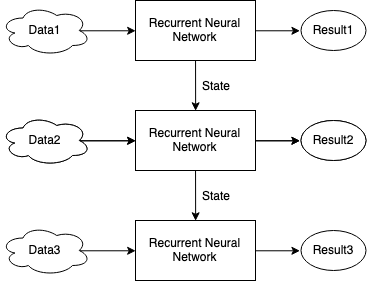
\includegraphics[width=300pt]{images/model_schema_5.png} \end{center}

Такое устройство сети в целом уже может удовлетворять основным нашим потребностям. Она умеет распознавать ключевые слова и способна последовательно обрабатывать различные синтаксические единицы, уделяя внимание контексту, образованному раннее.

Но мы пойдем дальше и будем использовать более сложноые, усовершенствованные рекуррентные сети под названием \textbf{LSTM} (от англ. \textit{Long short-term memory}).


\subsubsection{LSTM}
Усовершенствование заключается в введении механизмов управления памятью через регулирующие ее сущности, помогающие определить ценность информации для запоминания и фокусироваться только на тех вещах, которые нужны в текущий момент [1]. В литературе обычно говорят о трех таких механизмах:

\begin{itemize}
    \item \textbf{Forget gate} - механизм, определяющий подмноженство данных из долговременной памяти, которое необходимо забыть в текущем запуске.
    \item \textbf{Input gate} - механизм, определяющий подмножество данных, которое необходимо положить в долговременную память в текущем запуске.
    \item \textbf{Output gate} - механизм, определяющий подмножество данных из долговременной памяти, которое необходимо положить в кратковременную в текущем запуске.
\end{itemize}

Общепринятое название этих механизмов - \textbf{вентили}. Каждый из них реализован как сигмоида:

$$\sigma(x) = \frac{1}{1 + e^{-x}}$$

Используя внутреннюю память $c_t$, на каждом шаге работы сети вычисляется не только скрытое состояние $h_t$, но и вектор памяти $c_t$ [1]. Более подробные формулы вычисления вентилей:

$$f_t = \sigma(W_f x_t + U_f h_{t - 1} + b_f), ~i_t = \sigma(W_i x_t + U_t h_{t - 1} + b_i), ~ o_t = \sigma (W_o x_t + U_o h_{t - 1} + b_o)$$

Такой подход позволяет не зависеть от того, как давно была полученна важная информация. Если сеть видит, что она важна, она не будет забывать ее.

\subsubsection{BiLSTM}

Как можно понять, LSTM является итеративным алгоритмом, который проходит по словам в последовательном порядке. В качестве некоторого улучшения многие исследователи используют \textbf{бинаправленность} - добавляют к естественному порядку инвертированный. То есть, сеть проходит сначала слева направо, а потом справа налево. [5]

На практике такое решение дает некотороый прирост к качеству предсказаний.

\subsubsection{GRU}
Еще одна независимая от LSTM архитектура рекуррентных сетей называется \textbf{GRU} (от англ. \textit{Gated Recurrent Units}). Она была представлена в 2014 и отличается тем, что не содержит \textbf{Output gate}, а, значит, содержит на четверть меньше данных для обработки. [6]

В рамках этой работы мы только упомянем эту архитектуру и не будем глубоко погружаться в устройство ее работы.


\subsection{Постпроцессинг}

Выходом нейронной сети является некоторое вещественное число, которое с помощью операции \textbf{softmax} проецируется в отрезок [0, 1]. После этого наша задача найти такой порог определения в классы, при котором используемая в задаче F - мера покажет наилучший результат.


\pagebreak
	%% Спектр оператора
		\section{Реализация}

В этой главе я бы хотел порассуждать об архитектуре, через которую будет реализованно решение. На мой взгляд, очень часто ей уделяют недостаточно внимания. В то же время, от правильного планирования и реализации структуры проекта зависит его будущее. В моей практике встречается большое количество случаев, когда без своевременного продумывания архитектуры, компании годами сталкиваются с серьезными проблемами при поддержке и развитии легаси-кода.

\subsection{Общие соображения}
Как обычно выстраивается рабочий процесс, когда речь заходит о решении задачи по машинному обучению? В первую очередь в голову приходит довольно примитивная схема: есть некоторый пулл данных, для которых известен ответ (\textbf{Train}) и пулл, ответ для которого нужно предсказать (\textbf{ToPredict}). Мы загружаем первые данные в модель, обучаем ее, а затем получаем предсказание для данных второго типа. Представим эти соображения в виде схемы:

\begin{center} 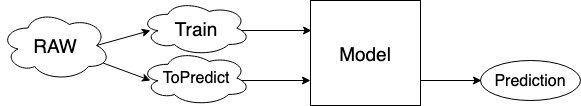
\includegraphics[width=350pt]{images/workflow_scheme_1}\end{center}

Следующим логическим развитием идеи будет добавление новой сущности для оценки качества модели (\textbf{ScoreCalculator}) и разделения известных данных на обучающие и тестовые (\textbf{Test}):


\begin{center} 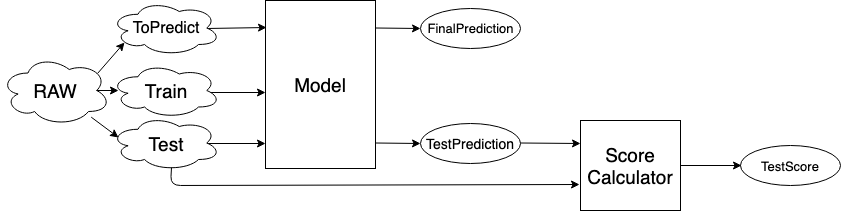
\includegraphics[width=450pt]{images/workflow_schema_2}\end{center}
Зачастую, с некоторыми небольшими вариациями, на этой схеме останавливаются. Мы же пройдем немного дальше.  Углубимся в детали, добавим некоторый новый расширяющий возможности функционал и постараемся сделать такую систему, которая бы легко масштабировалась на другие проекты, никак не связанные с нашей исходной задачей. 

\subsection{Усложняем структуру}
    
    В более сложных задачах данные требуют некоторой обработки (например, фильтрация, семплирование или преобразование в совершенно другую форму). Давайте в нашей диаграмме разделим данные на \textbf{XData},  \textbf{YData} и добавим сущность под названием \textbf{XTransformer}:
    
    \begin{center} 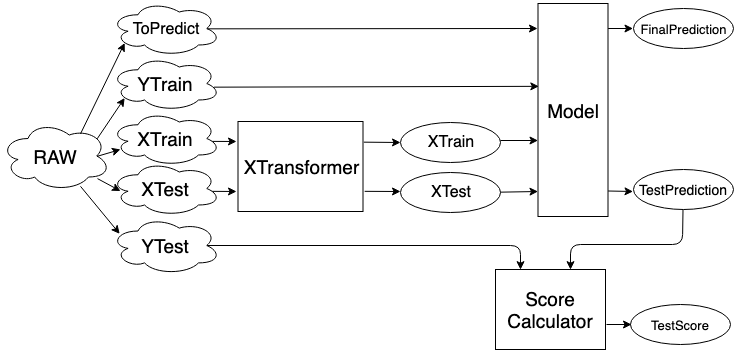
\includegraphics[width=450pt]{images/workflow_schema_3}\end{center}
    
    Еще одним нововведением предлагаю сделать сущность, которая бы отвечала за работу с сырыми данными: считывала, объединяла разные источники, разделяла на нужные выборки в нужном соотношении. Назовем ее \textbf{DataProvider}. По своему опыту могу судить о том, что такая инкапсуляция - одна из первых вещей, с которых стоит начинать развитие любого проекта, т.к. она освобождает основные алгоритмические сущности от управлением данных.
    
    \begin{center} 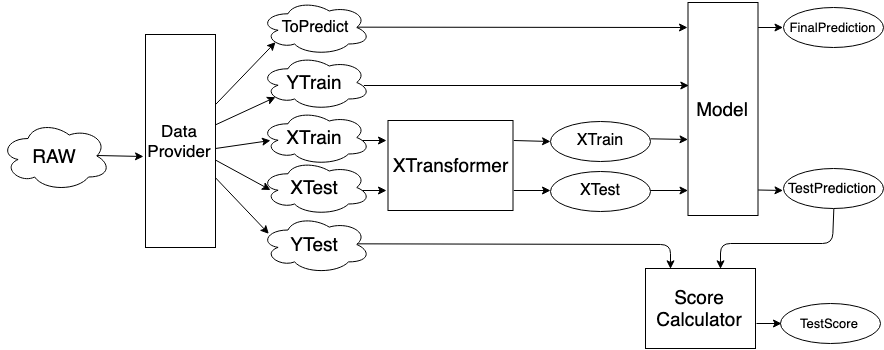
\includegraphics[width=450pt]{images/workflow_schema_4}\end{center}

    И завершающим элементом будет \textbf{Launcher} - точка входа в программу, которая является связующим звеном и реализует все связи, отображенные на схеме.
    
    
    \begin{center} 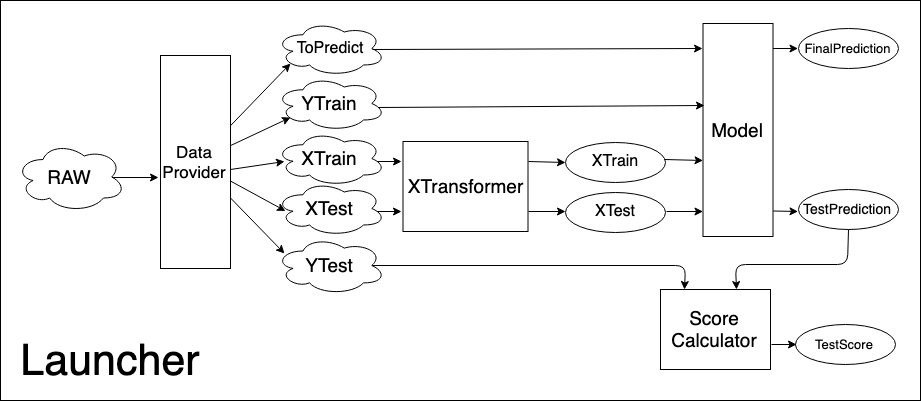
\includegraphics[width=450pt]{images/workflow_schema_5}\end{center}
    
    \pagebreak
    Выделим основные особенности архитектуры, которую мы получили:
    
    \begin{itemize}
        \item Не зависит от задачи, которая решается
        \item Состоит из независимых модулей, каждый из которых прост в реализации и решает одну определенную задачу
        \item Благодаря модульности, позволяет перебирать различные модели и трансформеры данных, чтобы подобрать оптимальные
        \item Легко добавить новые сущности, такие как композицию дополнительных моделей или визуализатор
    \end{itemize}
    
    
\pagebreak
\subsection{Техническая часть}
    
    В качестве языка программирования, на котором будет написан проект, очевидным выбором стал Python. Я начал с того, что в отдельном git репозитории реализовал структуру-каркас будущего решения, чтобы можно было взглянуть на разработанную архитектуру вне контекста решения задачи от Quora.
    
    Весь исходный код можно найти здесь: https://github.com/evgenstf/ml\_workflow.
    
    В рамках статьи мы не будем вдаваться в глубокие детали реализации, приведем лишь пару моментов, на которые стоит обратить внимание:
    
    \begin{itemize}
        \item \textbf{JSON конфиги}
        
     Всегда есть огромное количество констант, с которыми необходимо работать. От путей до данных и соотношения train/test до глубины решающего дерева и коэффициентов регуляризации. Мы будем держать их всех в одном месте: \textbf{config.json}, рядом с \textbf{launcher.py}. Для пустой реализации выглядит он следующим образом:
   \begin{lstlisting}[language=JSON]
{
  "data_provider": {
    "x_known": "../qdata/raw/simple_csv.csv",
    "y_known": "../qdata/raw/simple_csv.csv",
    "x_to_predict": "../qdata/raw/simple_csv.csv",
    "known_using_part" : 0.01, "train_part": 0.7
  },
  "x_transformer": {
    "name": "dummy"
  },
  "model": {
    "name": "dummy"
  },
  "answer_file": "answer.csv"
}
\end{lstlisting}

\pagebreak
    \item \textbf{Логгирование}
    
    Важнейшим аспектом разработки любого продукта является создание исчерпывающей системы логгирования. Мы будем поддерживать два режима: \textbf{DEBUG} и \textbf{INFO}.
    
    Ознакомиться с полным перечнем общеиспользуемых уровней логгирования и прочитать кейсы их применения можно вот здесь: \href{https://stackoverflow.com/questions/2031163/when-to-use-the-different-log-levels}{stackoverflow}.
    
    Пример информационного лога, который получается при запуске решения:
    \begin{lstlisting}[language=LOG]
INFO:Launcher:launcher config: {'x_transformer': {'name': 'w2v'}, 'model': {'loss_function': 'RMSE', 'l2_leaf_reg': 0.07, 'name': 'regboost', 'iterations': 1000, 'depth': 8, 'bootstrap_type': 'No', 'learning_rate': 0.2, 'classes_count': 5}, 'data_provider': {'x_to_predict': '../input/test.csv', 'known_using_part': 0.01, 'train_part': 0.8, 'x_known': '../input/train.csv', 'y_known': '../input/train.csv'}, 'embedding_provider': {'paragram_path': '../input/embeddings/paragram_300_sl999/paragram_300_sl999.txt', 'wiki_news_path': '../input/embeddings/wiki-news-300d-1M/wiki-news-300d-1M.vec', 'glove_path': '../input/embeddings/glove.840B.300d/glove.840B.300d.txt'}, 'answer_file': 'submission.csv'}
INFO:DataProvider:data provider config: {'x_to_predict': '../input/test.csv', 'known_using_part': 0.01, 'train_part': 0.8, 'x_known': '../input/train.csv', 'y_known': '../input/train.csv'}
INFO:DataProvider:loaded 13061 x_known lines
INFO:DataProvider:loaded 13061 y_known lines
INFO:DataProvider:loaded 56370 x_to_predict lines
INFO:DataProvider:splitted known data: x_train size: 10448 y_train size: 10448 x_test size: 2613 y_test size: 2613
INFO:DataProvider:inited
INFO:W2VXTransformer:x_transformer config:
INFO:W2VXTransformer:inited
INFO:W2VXTransformer:lemmatize called
\end{lstlisting}
    
	\end{itemize}
	
\subsection{Используемые библиотеки}

\subsubsection{Технические}

\begin{itemize}
    \item \textbf{json} - работа с JSON конфигами
    \item \textbf{logging} - логгирование
    \item \textbf{sys} - системные утилиты, такие как создание файлов, импорт из других дирикторий и т.п.
    \item \textbf{numpy} - упорядочивание данных, статистики, представления в виде таблиц
    \item \textbf{pandas} - надстройка над \textbf{numpy}, имеет в своем арсенале более продвинутые инструменты для исследований
    \item \textbf{sclearn} - набор метрик, инструменты для разделения данных на \textbf{train} и \textbf{test}
    \item \textbf{tqdm} - строка состояния обработки данных
\end{itemize}

\subsubsection{Препроцессинг}
\begin{itemize}
    \item \textbf{spacy} - инструменты для лемматизации и стеммизации слов
\end{itemize}


\subsubsection{Модель}
\begin{itemize}
    \item \textbf{keras.layers.LSTM} - реализация LSTM из библиотеки \textbf{keras}
    \item \textbf{keras.layers.Embedding} - работа с матрицей векторизации слов
    \item \textbf{keras.layers.Dropout} - реализация алгоритма \textbf{Dropout}, при котором удаляются случайные связи в сети для уменьшения переобучения.
    \item \textbf{keras.layers.Bidirectional} - бинаправленность в сети
\end{itemize}


\subsection{Результаты}

Лучший результат по F - мере, который мне удалось достичь используя векторизацию и LSTM - \textbf{0.63}. Можно сказать, что это скорее удачный результат, поскольку он показывает себя лучше, чем 70\% участников соревнования. 




 %% Сопряженный оператор
		
\section{Заключение}

В качестве итога проделанной работы предлагаю еще раз кратко закрепить то, к чему мы пришли в ходе нее.

Была рассмотрена задача об определении токсичного контента на портале знаний \textbf{Quora}. 

Мы осознали необходимость разработки гибкой архитектуры для более эффективного развития проекта. Такой подход позволил более четко обозначить части решения и написать их независимо друг от друга. 

После того, как наметилась структура проекта, была реализованна математическая модель, которая решает поставленную задачу. 

На выходе мы получили готовый сервис, который ввиду своей модульности легко можно разделить на микросервисы и внедрить в промышленный процесс компании.
 %% Последовательность ограниченных функций
		
\pagebreak
\section{Источники}

 [1] Фурин Н. Б. -- Методы извлечения терминологической информации на основе
машинного обучения. 2018

 [2] Tomas Mikolov, Kai Chen, Greg Corrado, and Jeffrey Dean -- Efficient estimation
of word representations in vector space. CoRR, abs/1301.3781

 [3] Tomas Mikolov, Ilya Sutskever, Kai Chen, Gregory S. Corrado, and Jeffrey Dean -- Distributed representations of words and phrases and their compositionality. In Advances in Neural Information Processing Systems 26: 27th Annual Conference on Neural Information Processing Systems 2013. Proceedings of a meeting held December 5-8, 2013, Lake Tahoe, Nevada, United States, pages 3111–3119, 2013
 
 [4] Jeffrey Pennington, Richard Socher, and Christopher D. Manning -- GloVe: Global Vectors for Word Representation. 2014
 
 [5] Christopher Olah -- Understanding LSTM Networks, 2014
 
 [6] Cho, Kyunghyun et al. -- Learning Phrase Representations using RNN Encoder-Decoder for Statistical Machine Translation. 2014
 
  %% Предел последовательности обобщенных функций (1)
		
	% предметный указатель %%%%%%%%%%%%%%%%%%%%%%%%%%%%%%%%%%%%%%%%%%%%%%%%%%%%%%
		%%% 
		%%% дополнительное (свое) задание верхнего	 колонтитула для предметного указателя
		%%% 
		
		%	\makeatletter
		%	\renewcommand{\@oddhead}{ \textcolor{blue}{Лекция (задача) \arabic{lections}} \hfil \par
		%	\hfil  \leftmark \hfil \rightmark }
		%	\makeatother
		% \printindex
	
\end{document}

%%
%%
%%
